\documentclass[xcolor=table]{beamer}

\usepackage[polish]{babel}
\usepackage[utf8]{inputenc}
\usepackage[T1]{fontenc}
\usepackage{listings}
\usepackage{lmodern}
\usepackage{textcomp}


\usetheme[language=polish]%
  {Goddard}

\newcommand{\filepath}{\texttt}
\newcommand{\command}{\texttt}
\newcommand{\email}[1]{\href{mailto:#1}{\texttt{#1}}}
\newcommand{\latexcode}{\texttt}
\newcommand{\parameter}[1]{\textlangle #1\textrangle}


\lstset{basicstyle=\ttfamily,keywordstyle=\color{goddardblue}\bfseries,commentstyle=\color{goddardblue!75}\itshape,columns=flexible}

\rowcolors{1}{goddardblue!50}{goddardblue!30}


\title{Metody rozpoznawania twarzy}
\subtitle{przeglad i porównanie}
\author{Bartłomiej Bułat\\
Tomasz Czarnik\\
Krzysztof Śmiłek\\}


\begin{document}

\begin{frame}
  \titlepage
\end{frame}


\begin{frame}
  \frametitle{Plan}
  \tableofcontents
\end{frame}


\section{Wstęp}

\begin{frame}
  \frametitle{Wstęp}
  Rozpoznawanie twarzy to najbardziej naturalny sposób identyfikacji osób. Wraz z rozwojem technologii i mocy obliczeniowej szuka się coraz doskonalszych rozwiązań uskuteczniających to zadanie.\\[\baselineskip]
\uncover <2-> {Przykładowe zastosowania:
\begin{itemize}
\item Fotografia cyfrowa
\item Metody autoryzacji
\item Bezpieczeństwo w strefie publicznej
\item Rozrywka (konsole nowej generacji)
\end{itemize}}
\end{frame}

\subsection{Problem i ogólny algorytm}
\begin{frame}
  \frametitle{Problem rozpoznawania twarzy}
    01:04 póżno już, idę spać\\tsm
\end{frame}
\begin{frame}
  \frametitle{Ogólny algorytm}
   
\end{frame}


\section{Metody rozpoznawania twarzy}

\subsection{Metody geometryczne}
\begin{frame}
  \frametitle{Metody geometryczne}

  dodać info o metodzie

\end{frame}

\begin{frame}
  \frametitle{Metody geometryczne}

  a to jest drugi slajd geometrycznych etc

\end{frame}

\subsection{Metoda analizy kolorów}
\begin{frame}
  \frametitle{Metoda analizy kolorów}

  dodać info o metodzie

\end{frame}

\subsection{Metoda sieci neuronowych}
\begin{frame}
  \frametitle{Metoda sieci neuronowych}

  dodać info o metodzie

\end{frame}

\subsection{Model aktywnego kształtu}
\begin{frame}
  \frametitle{Model aktywnego kształtu}
  \begin{itemize}
  \uncover <1-> {\item Idea opracowana w 1995 roku przez Tim Cootesa oraz Chrisa Taylora}
  \uncover <2-> {\item Model statyczny, który "próbuje" dopasować się do obiektu na obrazie}
  \uncover <3-> {\item Wzorzec określany przez rozkład punktów}
  \uncover <4-> {\item Proces uczenia polega na zaznaczeniu punktów twarzy na wielu zdjęciach testowych}
  \uncover <5-> {\item Otrzymane wektory normalizuje się, po czym na podstawie średniego kształtu, odchylenia od średniej i macierzy kowariancji wyznaczony zostaje model}
 \end{itemize}
\end{frame}

\begin{frame}
  \frametitle{Model aktywnego kształtu - maska}
\begin{center}
  \begin{figure}
    \only<1> {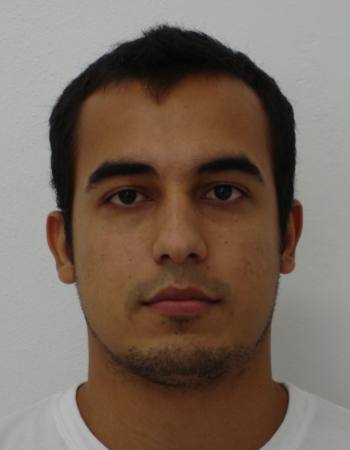
\includegraphics[scale=0.4]{aktywny2.png}}
    \only<2> {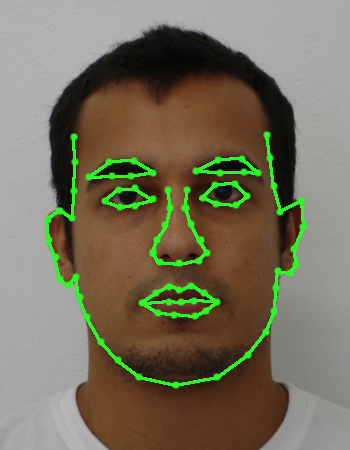
\includegraphics[scale=0.4]{aktywny3.png}}
    \only<3> {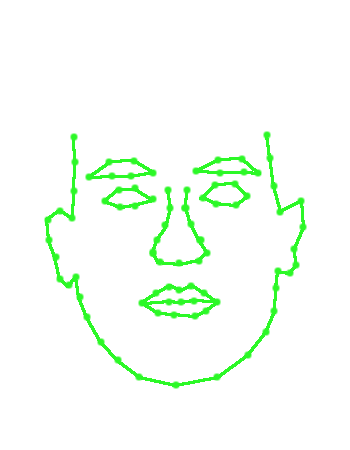
\includegraphics[scale=0.4]{aktywny1.png}}
    \caption{Przykład dopasowania maski}
  \end{figure}
\end{center}
\end{frame}

\begin{frame}
  \frametitle{Model aktywnego kształtu \\ - lista kroków wyszukiwania obiektu}
  \begin{itemize}
\item Badane jest sąsiedztwo każdego punktu charakterystycznego w poszukiwaniu odpowiedniej deformacji
\item Obliczane są optymalne parametry przesunięcia, obrotu, skali tak aby umieścić niezdeformowany model jak najbliżej rzeczywistego kształtu
\item Uważając na dopuszczalny zakres zmian uaktualnia się parametry modelu dopasowując go jak najdokładniej do obrazu
\item Przesunięcie punktów charakterystycznych na podstawie krawędzi prostopadłych do brzegu modelu oraz poziomów jasności
\end{itemize}
\end{frame}

\begin{frame}
  \frametitle{Model aktywnego kształtu - podsumowanie}
   \uncover <1-> { Zalety:
\begin{itemize}
\item Duża elastyczność - model potrafi dopasować się do różnych kształtów
\item Uniwersalny - kształt określany jest w drodze uczenia
\item Pomocny przy klasyfikowaniu i identyfikowaniu twarzy
\end{itemize}
}
  \uncover <2-> {\noindent 
Wady:
\begin{itemize}
\item  Czasochłonne i trudne uczenie modelu 
\item  Mało odporny na zmieniające się warunki oświetlenia, zróżnicowanego tła, bardziej realistycznych warunków
\item  Słabe wyniki dla osób z długimi ciemnymi włosami
\end{itemize}}
\end{frame}
\section{Porównianie}

\begin{frame}
  \frametitle{Porównanie}

  porównanie

\end{frame}

\section{Podsumowanie}

\begin{frame}
  \frametitle{Podsumowanie}

  parę słów podsumowania tutaj

\end{frame}



\end{document}
